\documentclass[12pt]{article}
\usepackage[utf8]{inputenc}
\usepackage{amssymb}
\usepackage{wasysym}
\usepackage[a4paper, margin=2cm]{geometry}
\usepackage[T1]{fontenc}
\usepackage{CJKutf8}
\usepackage[dvipsnames]{xcolor}
\usepackage{graphicx}
\graphicspath{ {./images/} }
\usepackage{scrextend}
\usepackage{hyperref}
\hypersetup{colorlinks=true,
            linkcolor=blue,
            filecolor=magenta,      
            urlcolor=cyan,}
\urlstyle{same}

\title{\textbf{Proof of Concept - Elaboration II: Testing and Revision}}
\date{08 Oct 2019}
\author{William Black 42920477}
\setlength{\parindent}{0pt}
\setlength{\parskip}{0.5em}

\begin{document}

\underline{\textbf{\Large{Formatting Tests}}}

\section{\large Format any LaTeX section label to be grey and bold.}

\textbf{Intention:} Based on my own new skills in LaTeX, I think I should be able to apply standard formatting to section labels.

\textbf{Action:} In a new sample LaTeX document, applying the normal to the section heading. \vspace{-0.5em}\begin{verbatim}
\section{\textbf{\textcolor{gray}{Section Title Here}}}    \end{verbatim}\vspace{-0.5em}

\textbf{Result:} It works, but leaves the number black. 

\textbf{Action:} Trying it the other way around
\vspace{-0.5em}\begin{verbatim}
\textcolor{gray}{\subsection{\textbf{Section Title Here}}}  \end{verbatim}\vspace{-0.5em}

\textbf{Result:} Test successful. This is good to keep in mind formatting can be applied to only word-count though, as some sections would not be greyed out.

\section{\large Create macro that applies that formatting to all section headings.}

\textbf{Intention:} Use \href{https://en.wikibooks.org/wiki/LaTeX/Creating_Packages}{this tutorial} to make a .cls class or .sty package. The page says "They are very similar, the main difference being that you can load only one class per document." Brian suggests I might make a .sty package, since I'm \textit{not} attempting to make a stylistic rendering of a document.

The instructions then say to write a document preamble to make the macro, and save it in a .sty file.

Using a real essay that I'm currently writing, I'll copy the code for the headings with word counts that I've been typing out by hand so far, and create a file called \texttt{pocgoal.tex} to keep track of the goal. Then I'll write three instructions, one each for sections, subsections, and subsubsections, that applies formatting to two arguments - which will be the heading and the word count separately.

\newpage\textbf{Action:} 

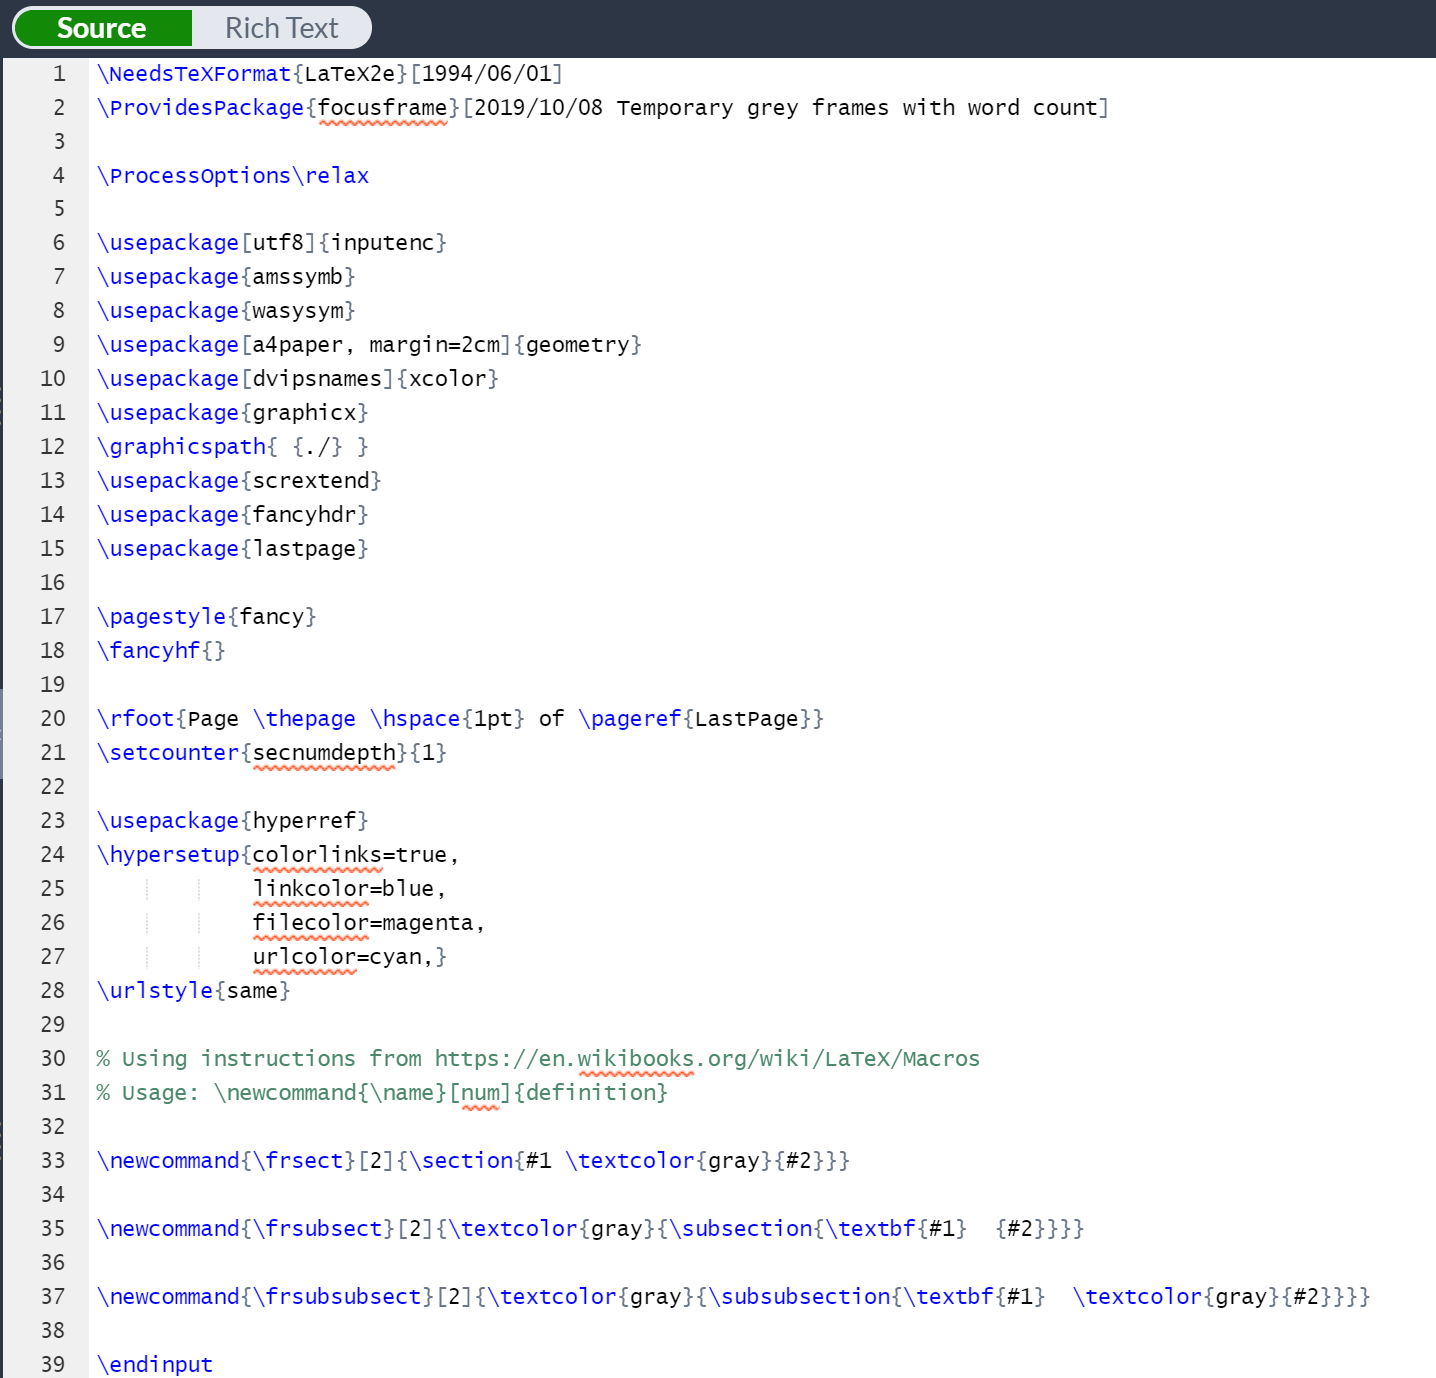
\includegraphics[scale=0.5]{imgfrstyfile.png}

\textbf{Result:} 

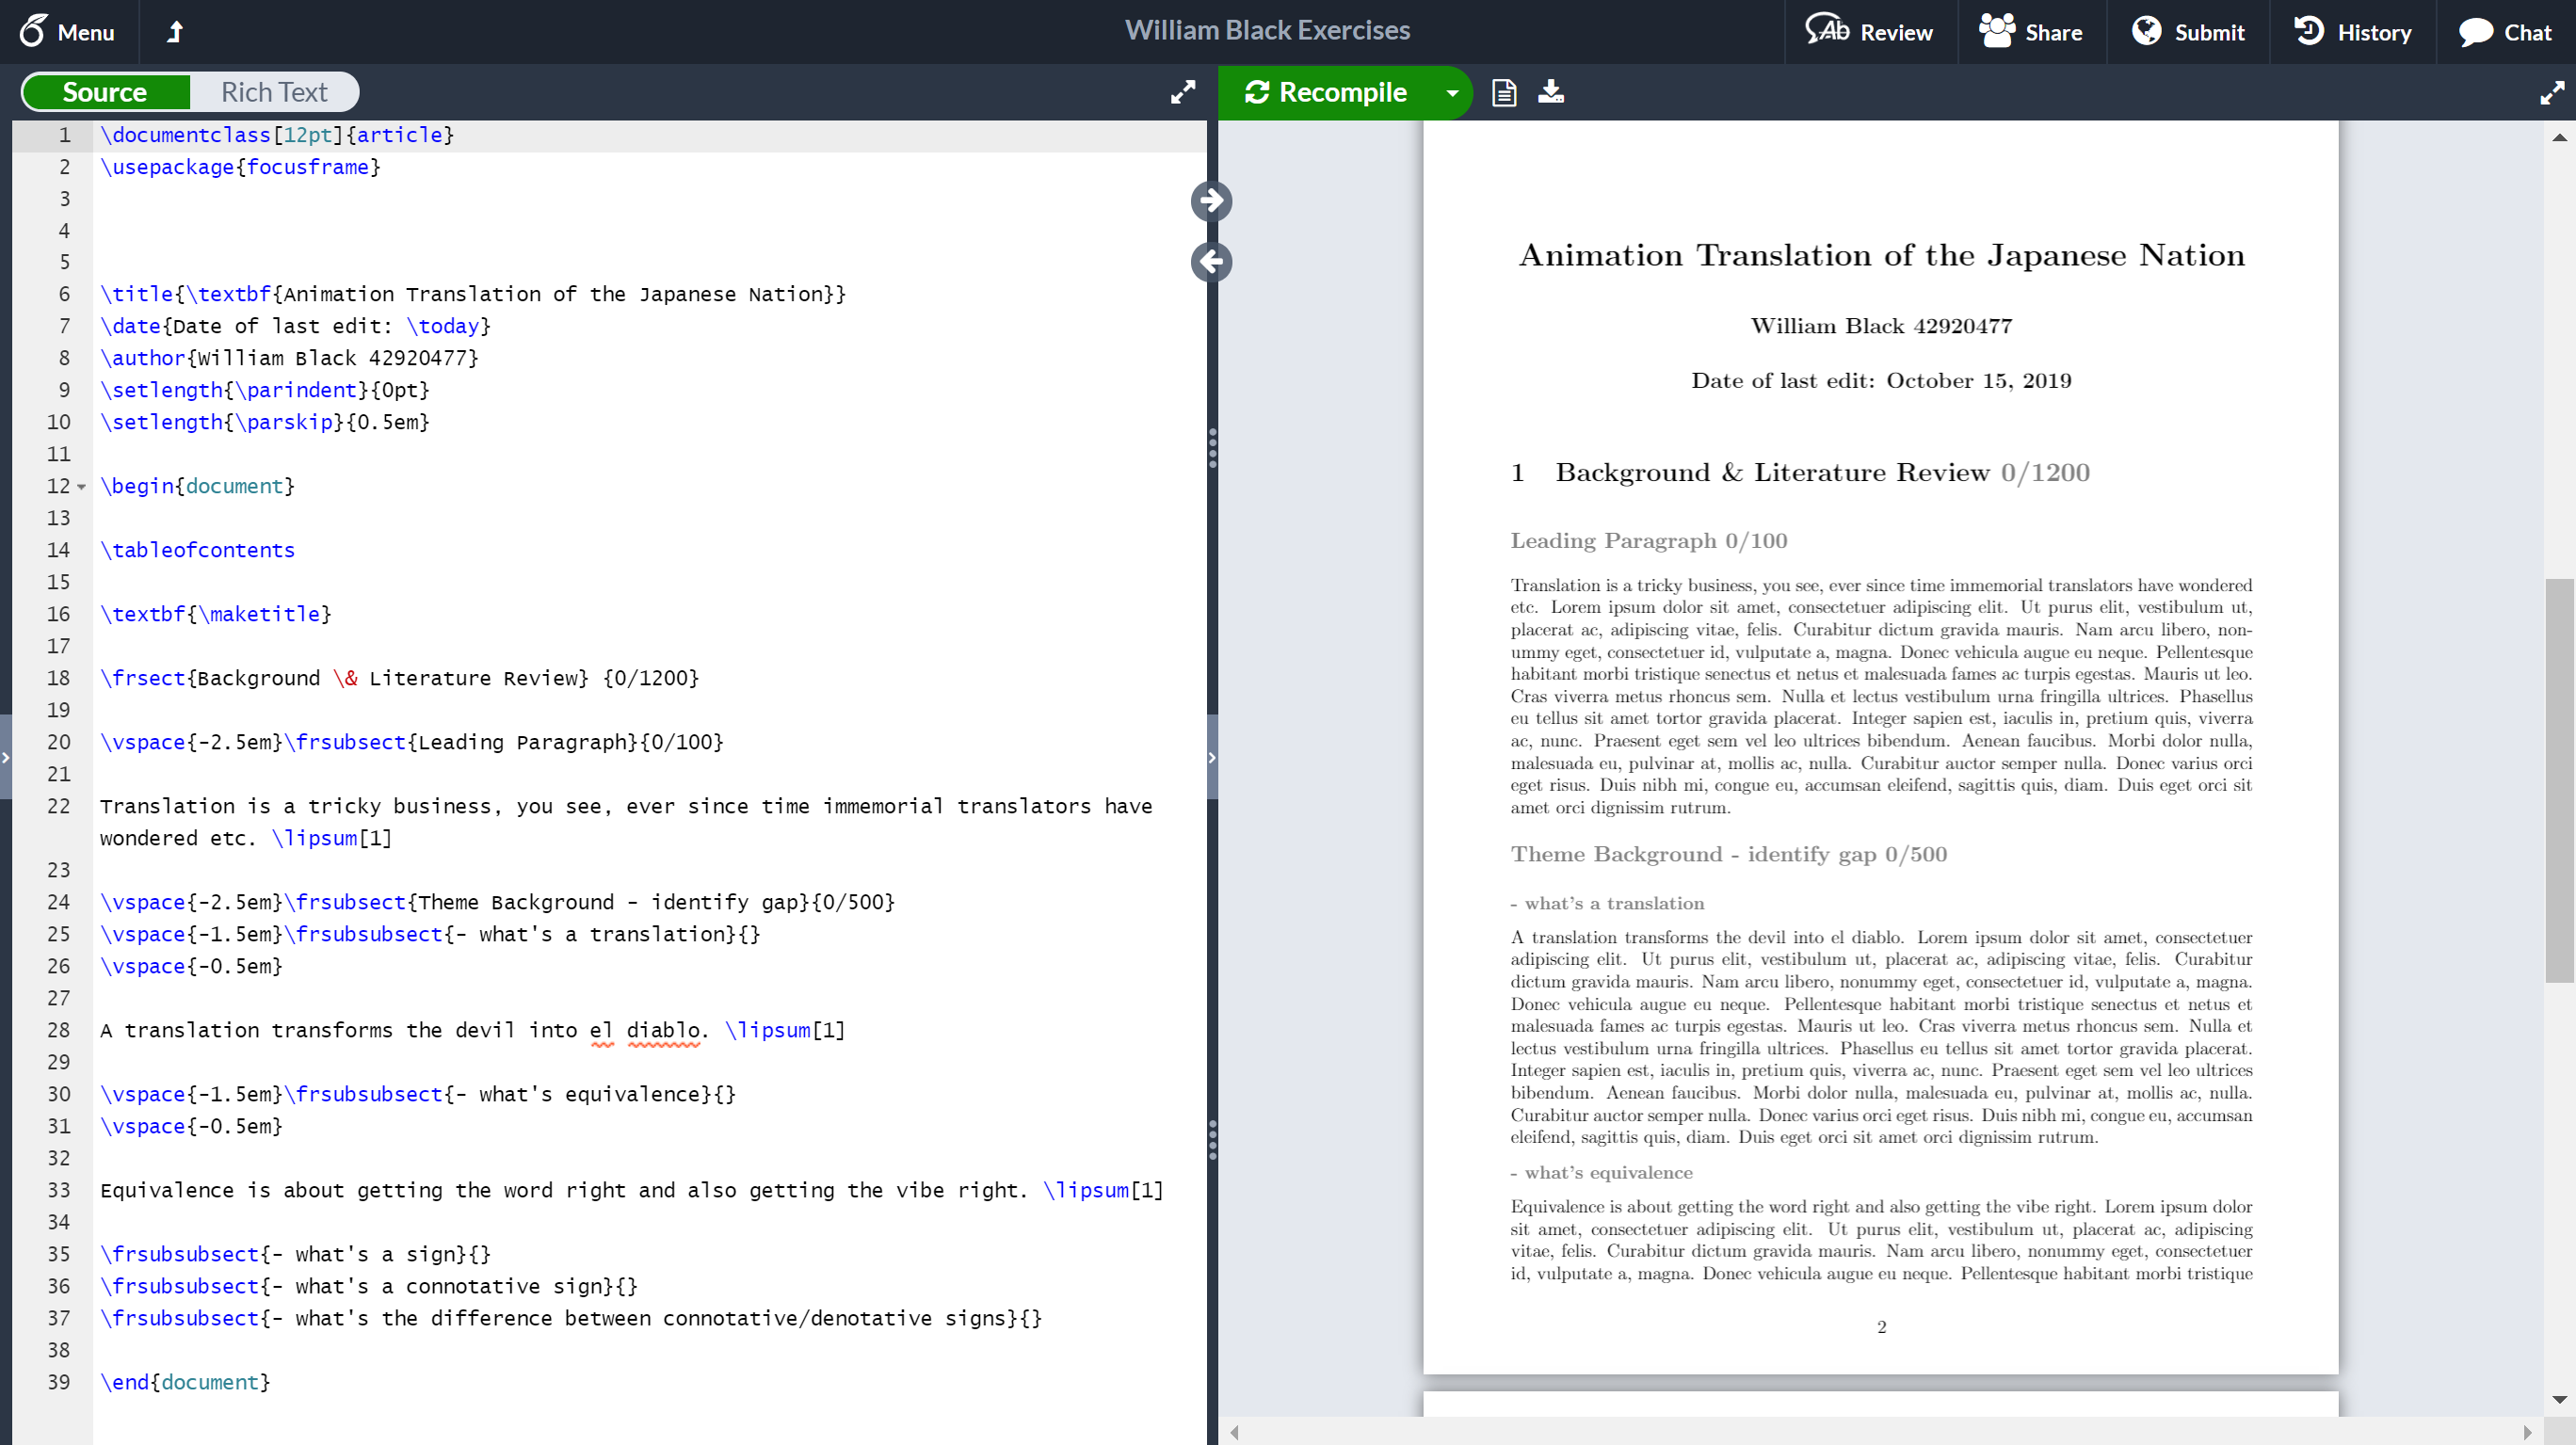
\includegraphics[width=\textwidth]{imgfrvspace.PNG}

The headings and word counts are applying, but I realised I need to change the vertical space to a negative integer to keep a balanced look in the document. It would be easier to add this to the .sty file, as it will always look better with the space I've manually written in.

\newpage\textbf{Action:} 

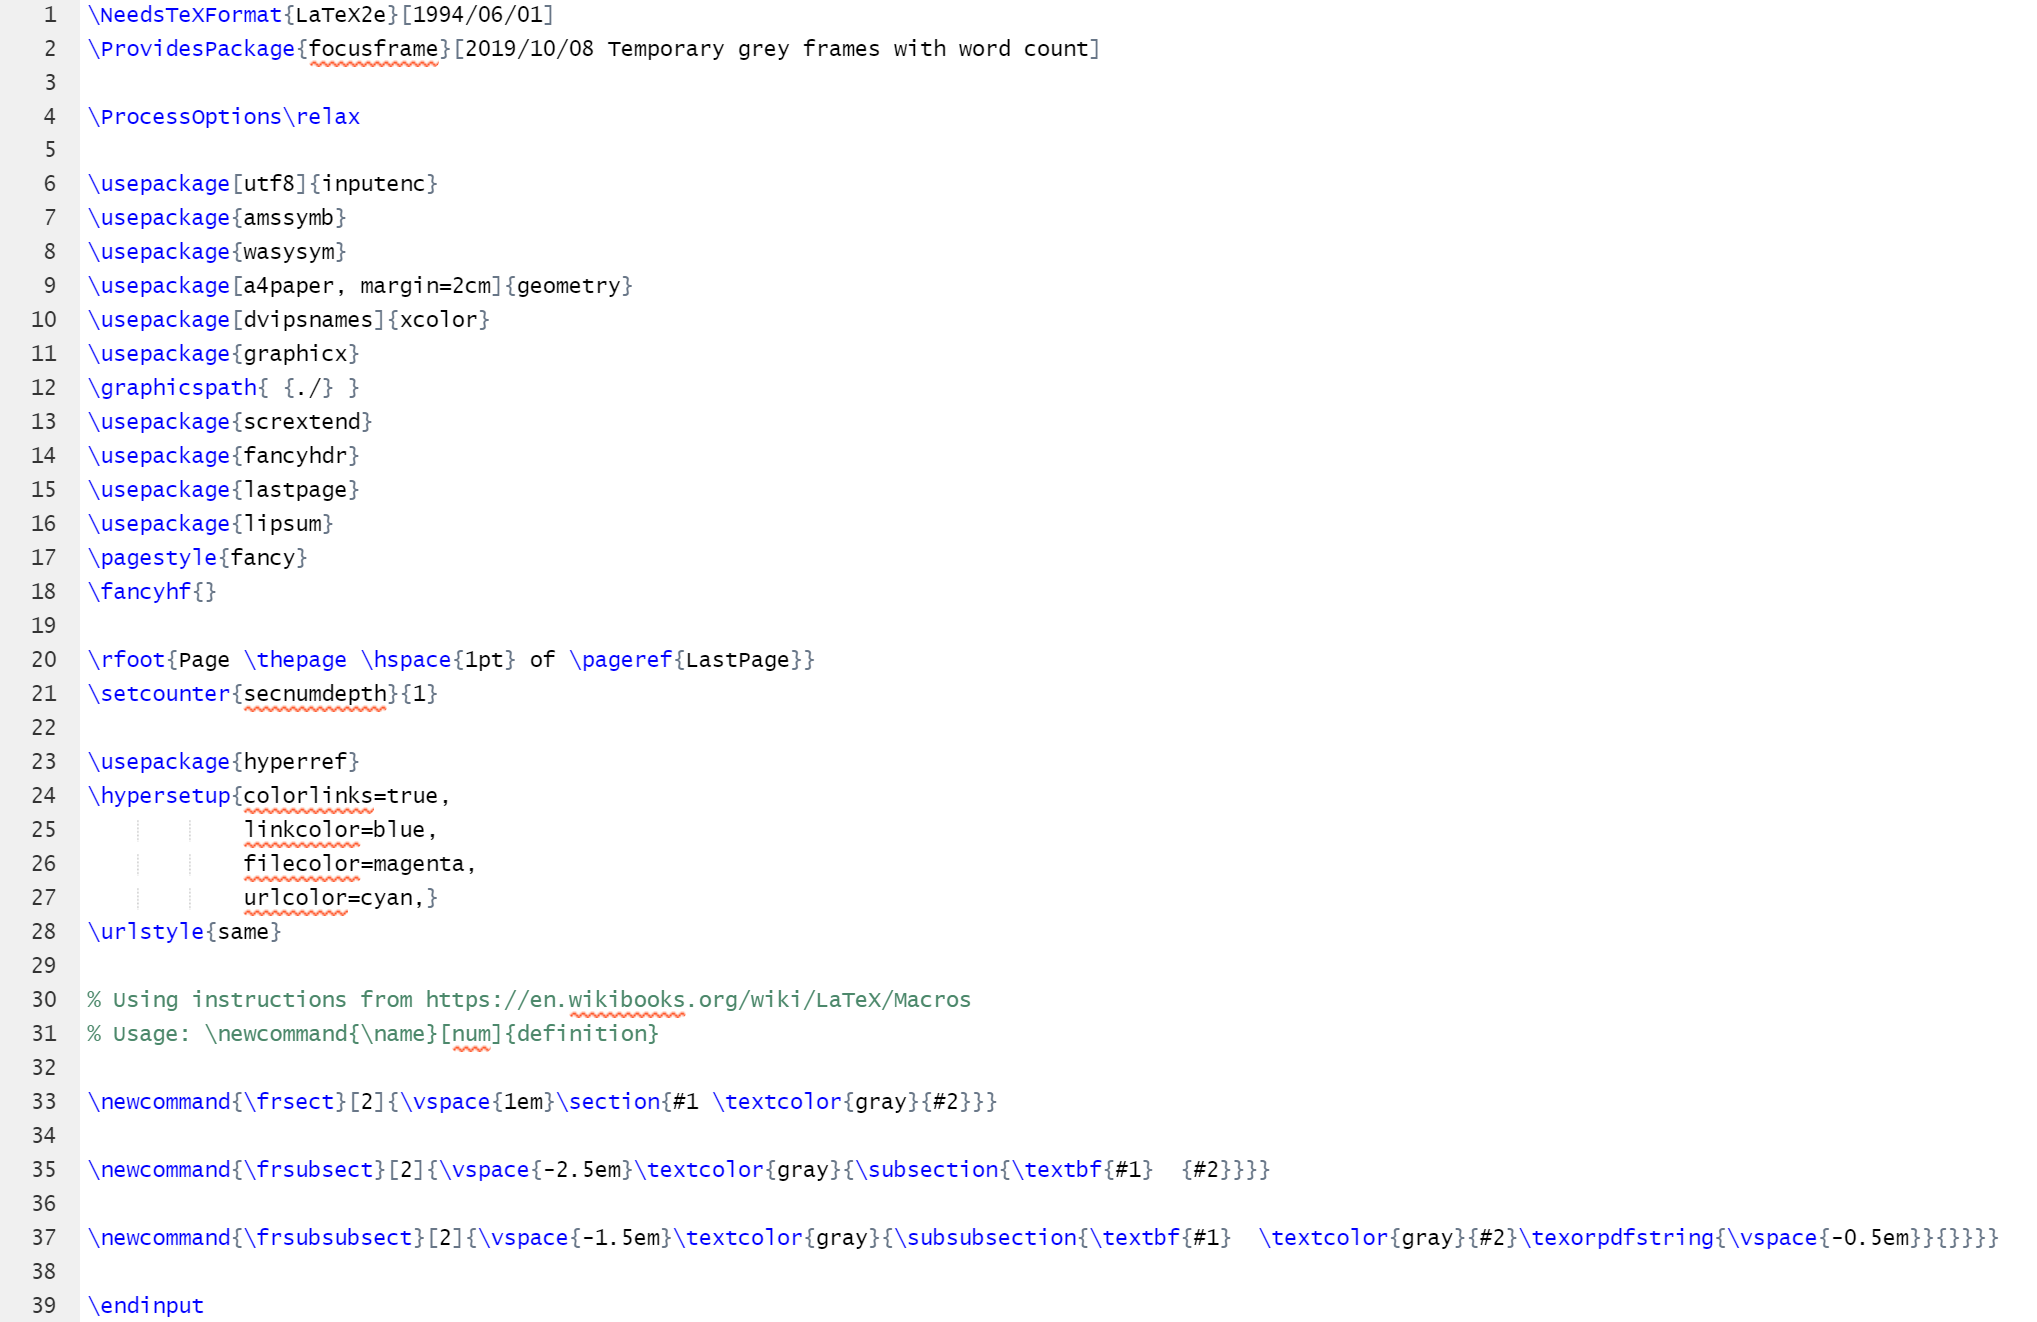
\includegraphics[scale=0.5]{imgfrstyfile2.PNG}

\textbf{Result:} 

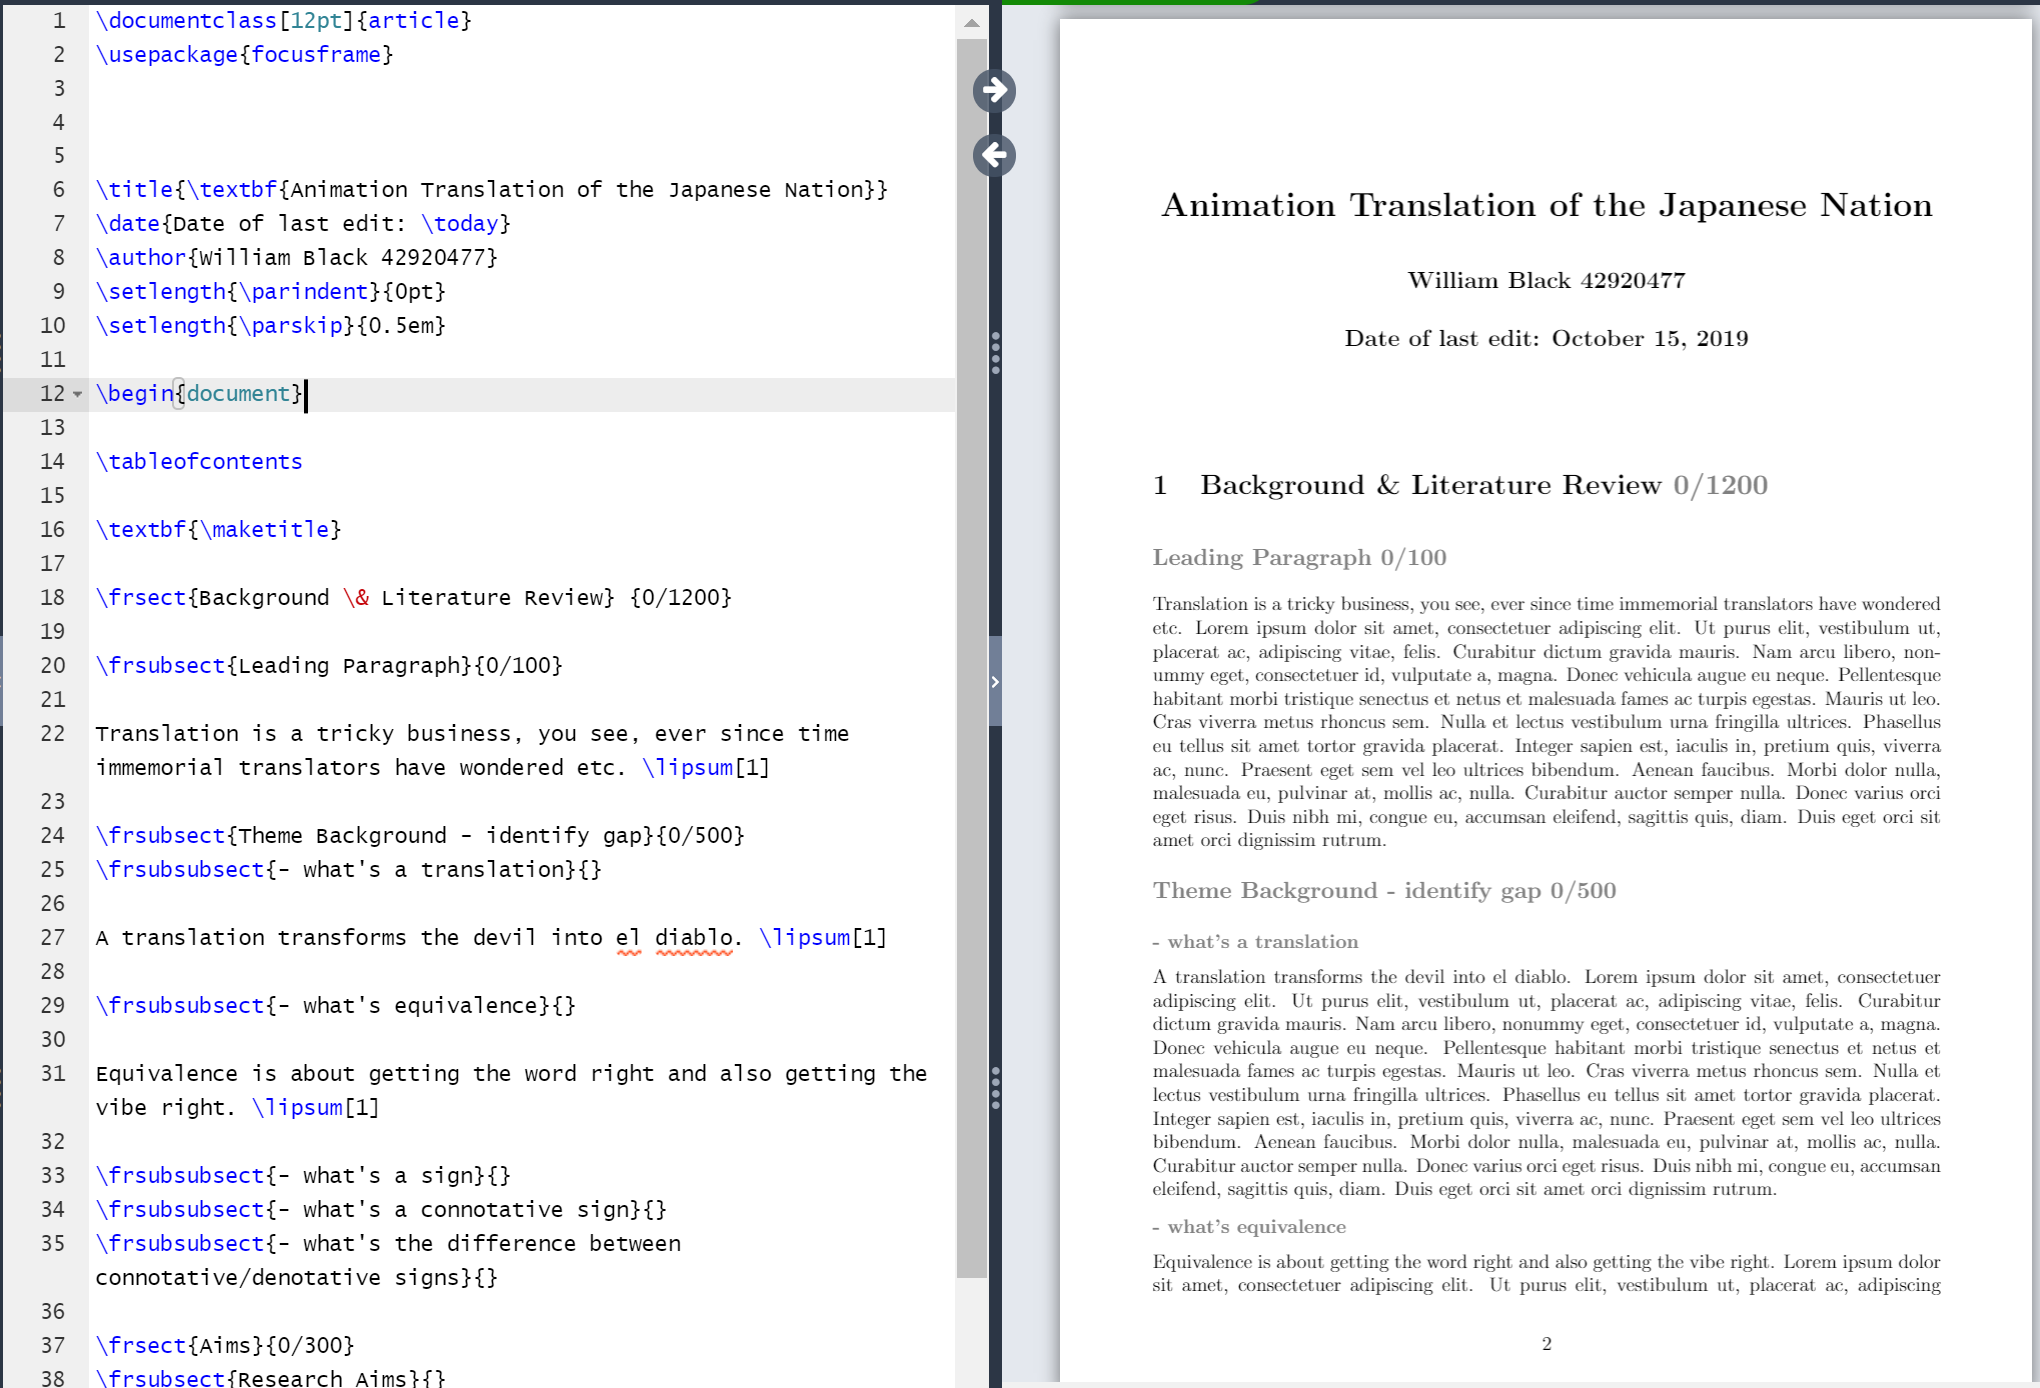
\includegraphics[width=\textwidth]{imgfrvspace2.PNG}

\section{\large Apply macro to all sections, subsections and subsubsections.}

This was inadvertently accomplished during the last test. Formatting was applied by macro, and no longer needs to be applied to sectioning system since the commands already contain sectioning instructions.

\newpage

\underline{\textbf{\Large{Word Count Tests}}}
\section{\large Add word count goal to formatting macro}

\textbf{Intention:} To add argument to section title macro to allow a word count goal to be placed next to section title.

\textbf{Action:} \begin{verbatim}
    \newcommand{\frsect}[2]{%
        \textcolor{gray}{\textbf{#1/ #2 words}}%
        }
\end{verbatim}

\textbf{Result:} The second argument as the word count goal is functional. The first argument will be replaced by the extracted subcount of the section.

\section{\large Extract subcount of words in LaTeX}

\textbf{Intention:} After much research and eventually tuition, it appears that my intention should be to use the LaTeX shell to echo my desired result from the \texttt{texcount} package.

The package comes with more detail than I want to include, so I will grep the line I need from the document and create a separate section count file, so I can cut the first field using the second character as a delimiter, to extract only the number of words in the main text.

\textbf{Action:} 

\begin{verbatim}
    \newcommand{\texcountnobibsinglefile}[1]{%
        \immediate\write18{texcount -sum -subcount #1.tex > texcou.nt}%
        }
    \newcommand{\getsectioncount}[2]{%
        \texcountnobibsinglefile{WilliamBlack-poctest}
        \immediate\write18{grep "#1" texcou.nt > sectcou.nt}
        \immediate\write18{cut -d + -f 1 sectcou.nt > cleancou.nt}
        \input{cleancou.nt}#2 words%
        }
\end{verbatim}

\textbf{Result:}

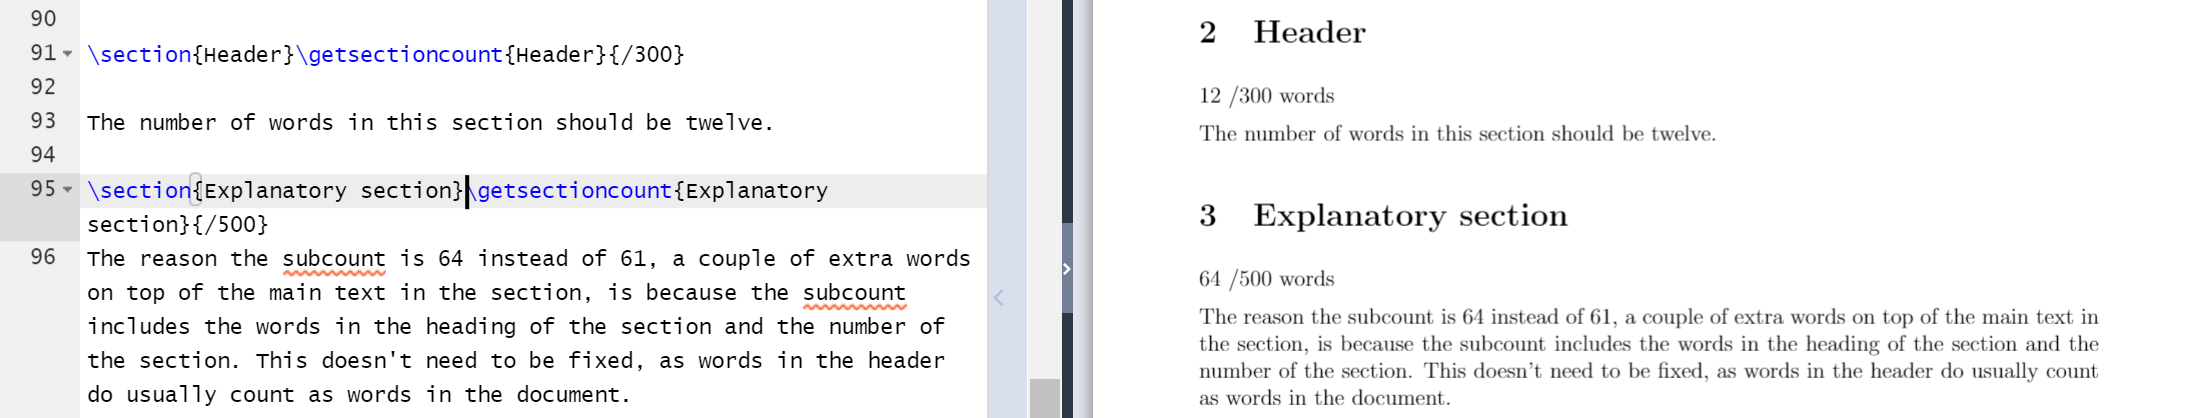
\includegraphics[width=\textwidth]{imgelaborationsubcountworks.PNG}

It does work, but there are a few unresolved issues:

\begin{enumerate}
    \item The counts include words in the heading of the section, and the number of the section, as words in the main text. That's okay because it's usually a small number, but technically, a lot of the headings will disappear in the final product, so shouldn't be counted.
    \item I have to write the name of the file I want to do this to every time. I think there should be a way to input this automatically, as this preamble will eventually go in the .sty file.
    \item The resulting word count in cleancou.nt gets pulled with a space automatically following it. This is more or less okay, despite being unexpected. Unfortunately, it also adds itself as a new line and I would have to manipulate cleancou.nt in order to keep it in line with the frame. Not sure how to do that yet.
\end{enumerate}

\textbf{Solutions:}
\begin{enumerate}
    \item I've realised the easiest way to handle this is to simply delete wordy headings when they're no longer needed. I was envisioning headings such as "short description of issues faced by users when access to tools is impeded by network breakdown - 0/200 words", which would eat into the word count. Once I've written the body of such summarising headings to approach the wordcount goal, there's no need for them to stay.
    \item I found \href{https://tex.stackexchange.com/questions/6990/what-is-the-variable-that-contains-the-source-file-name}{a command} that will act as the name of the current file in all LaTeX documents. It doesn't work in Overleaf, because \texttt{$\backslash$jobname.tex} always shows "\texttt{output.tex}". Hours of searching have provided no workaround for Overleaf, so I could either use a different platform, or just allow my tool to require defining \texttt{$\backslash$xjobname.tex} in the preamble.
    \item Thankfully, before trying to mess with cleancou.nt with another macro, I realised I could insert the input into the section title.
\end{enumerate}

\section{\large Apply subcount to all levels of sectioning}

\textbf{Intention:} Because the current subcount only works for subsections, applying it to sections only provides "3 words" - the two-word title and the section number - as it is immediately followed by the next subsection heading. As suspected, a separate macro will need to be made per section hierarchy.

\textbf{Action:}

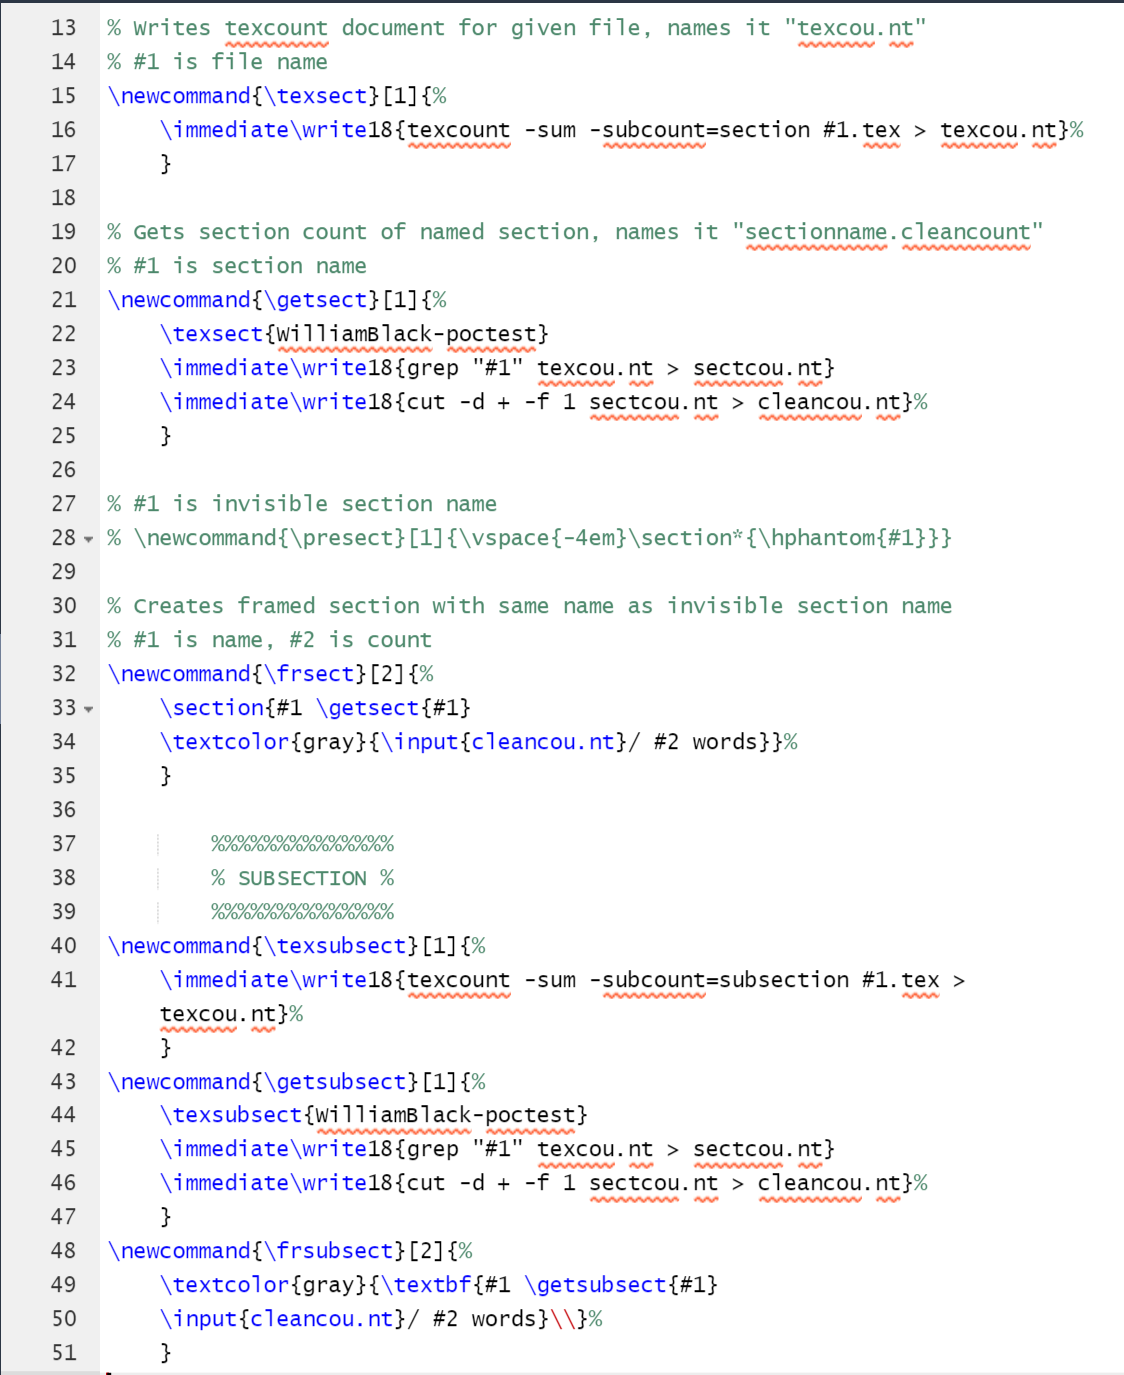
\includegraphics[scale=0.9]{imgelaborationsubsectcount.PNG}

\textbf{Result:} This correctly provides subcounts for sections and subsections, but is not a usable code to find the total sum of words used in the file. A new macro will need to be made for that purpose. 

Using \texttt{texcount} package does not allow counts for subsubsections, and after further tinkering, I have noted that finding a work-around for this would not save me enough time to be worth learning a new skill. I am happy enough with this tool without requiring a subsubsection count.

\textbf{Action:}
\begin{verbatim}
    \newcommand{\texfile}[1]{%
        \immediate\write18{texcount -sum -subcount=none #1.tex > texcou.nt}}
    
    \newcommand{\getfile}{\texsect{WilliamBlack-poctest}
        \immediate\write18{grep "Sum" texcou.nt > filecou.nt}
        \immediate\write18{cut -d : -f 2 filecou.nt > cleancou.nt}}

    \newcommand{\frfile}[1]{%
        \textcolor{gray}{\getfile\input{cleancou.nt}/ #1 words}}
\end{verbatim}

\textbf{Result:}

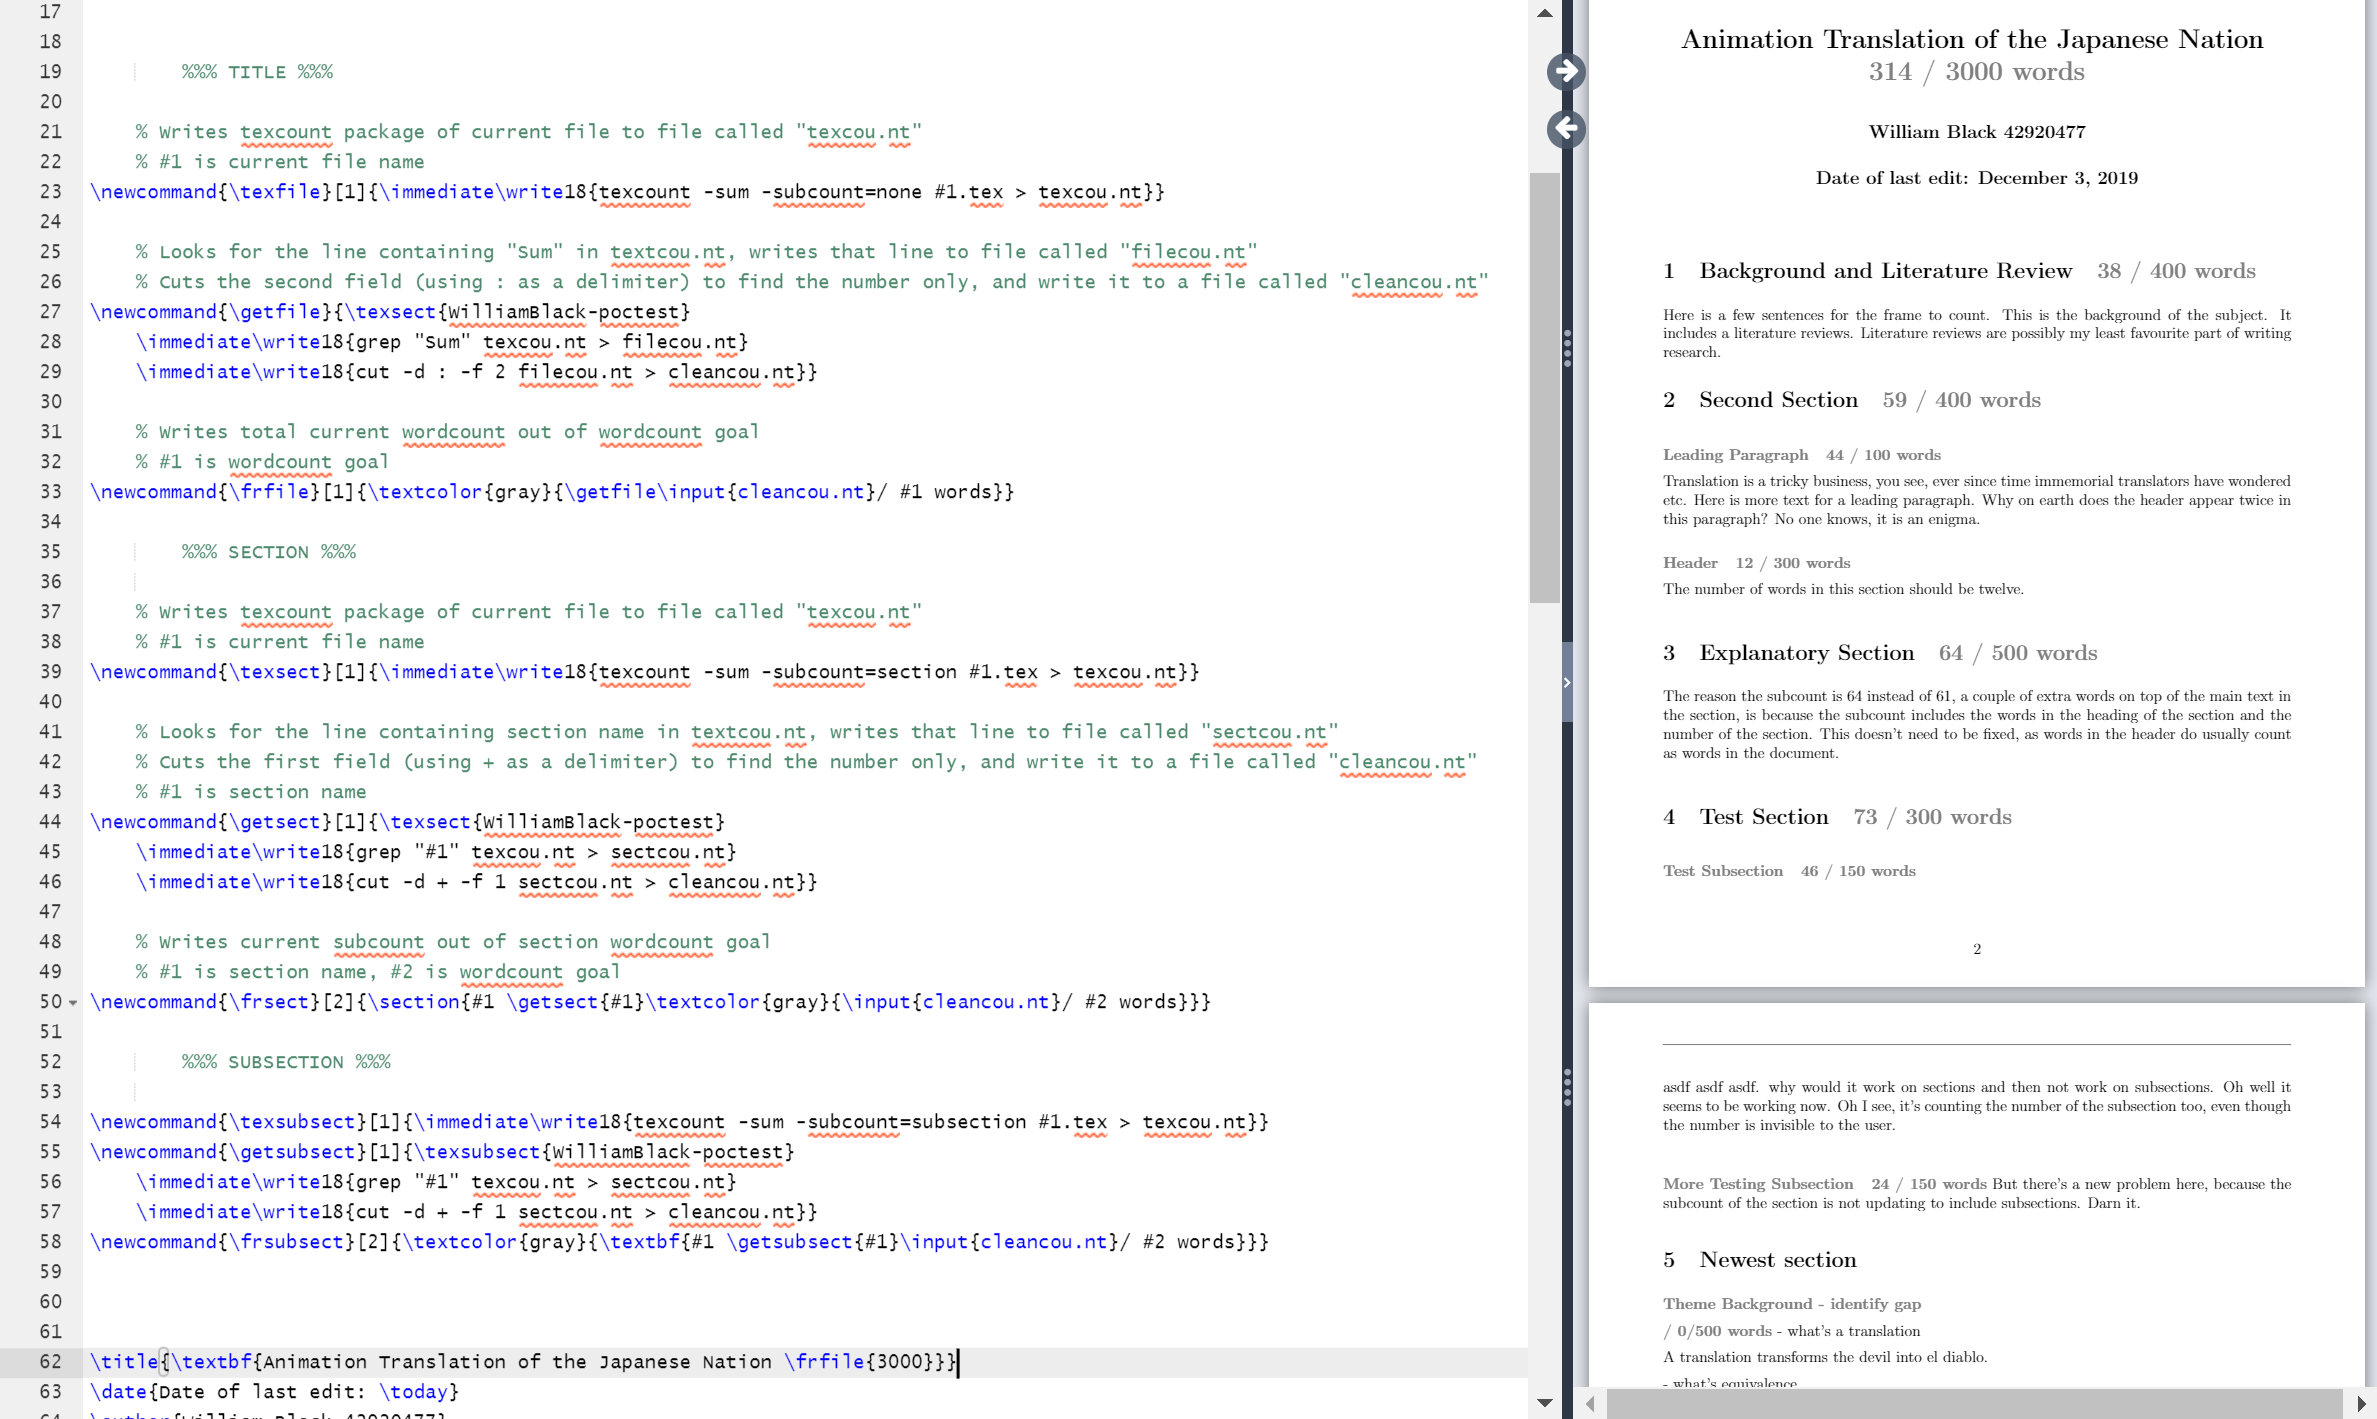
\includegraphics[width=\textwidth]{imgelaborationfullcountsubcount.PNG}

The only problem I'm having with this is that in the actual document, I have to write 
\begin{verbatim}
    \vspace{-3em}\subsection*{\hphantom{Header}}

    \frsubsect{Header}{300}
\end{verbatim}
This is because the macro doesn't seem to be able to create the section and THEN run the search on what it created. The phantom section is created so that the macro has it to search for. I can't stick these two lines into a new command either, because the new command will still run them simultaneously.

\textbf{Action:}

According to the TeXCount \href{https://app.uio.no/ifi/texcount/download.php?doc=TeXcount_3_1_1.pdf}{instructions}: 

"subst macro text This substitutes a macro with any text. The verbose output will show the substituted text: e.g. \%TC:subst $\backslash$test TEST will cause a following $\backslash$newcommand$\backslash$test{TEST} to be changed into $\backslash$newcommand TEST{TEST}, which TEXcount will interpret differently. Use with care!"

So I use \texttt{\%TC:subst frsect section} to substitute frsect for section within the code, which allows TeXCount to function correctly, but also keeps my macro working.

\textbf{Result:}

It's functioning correctly at all levels now. At Brian's suggestion, the macro now uses margins to show the word count to be easier to scan.

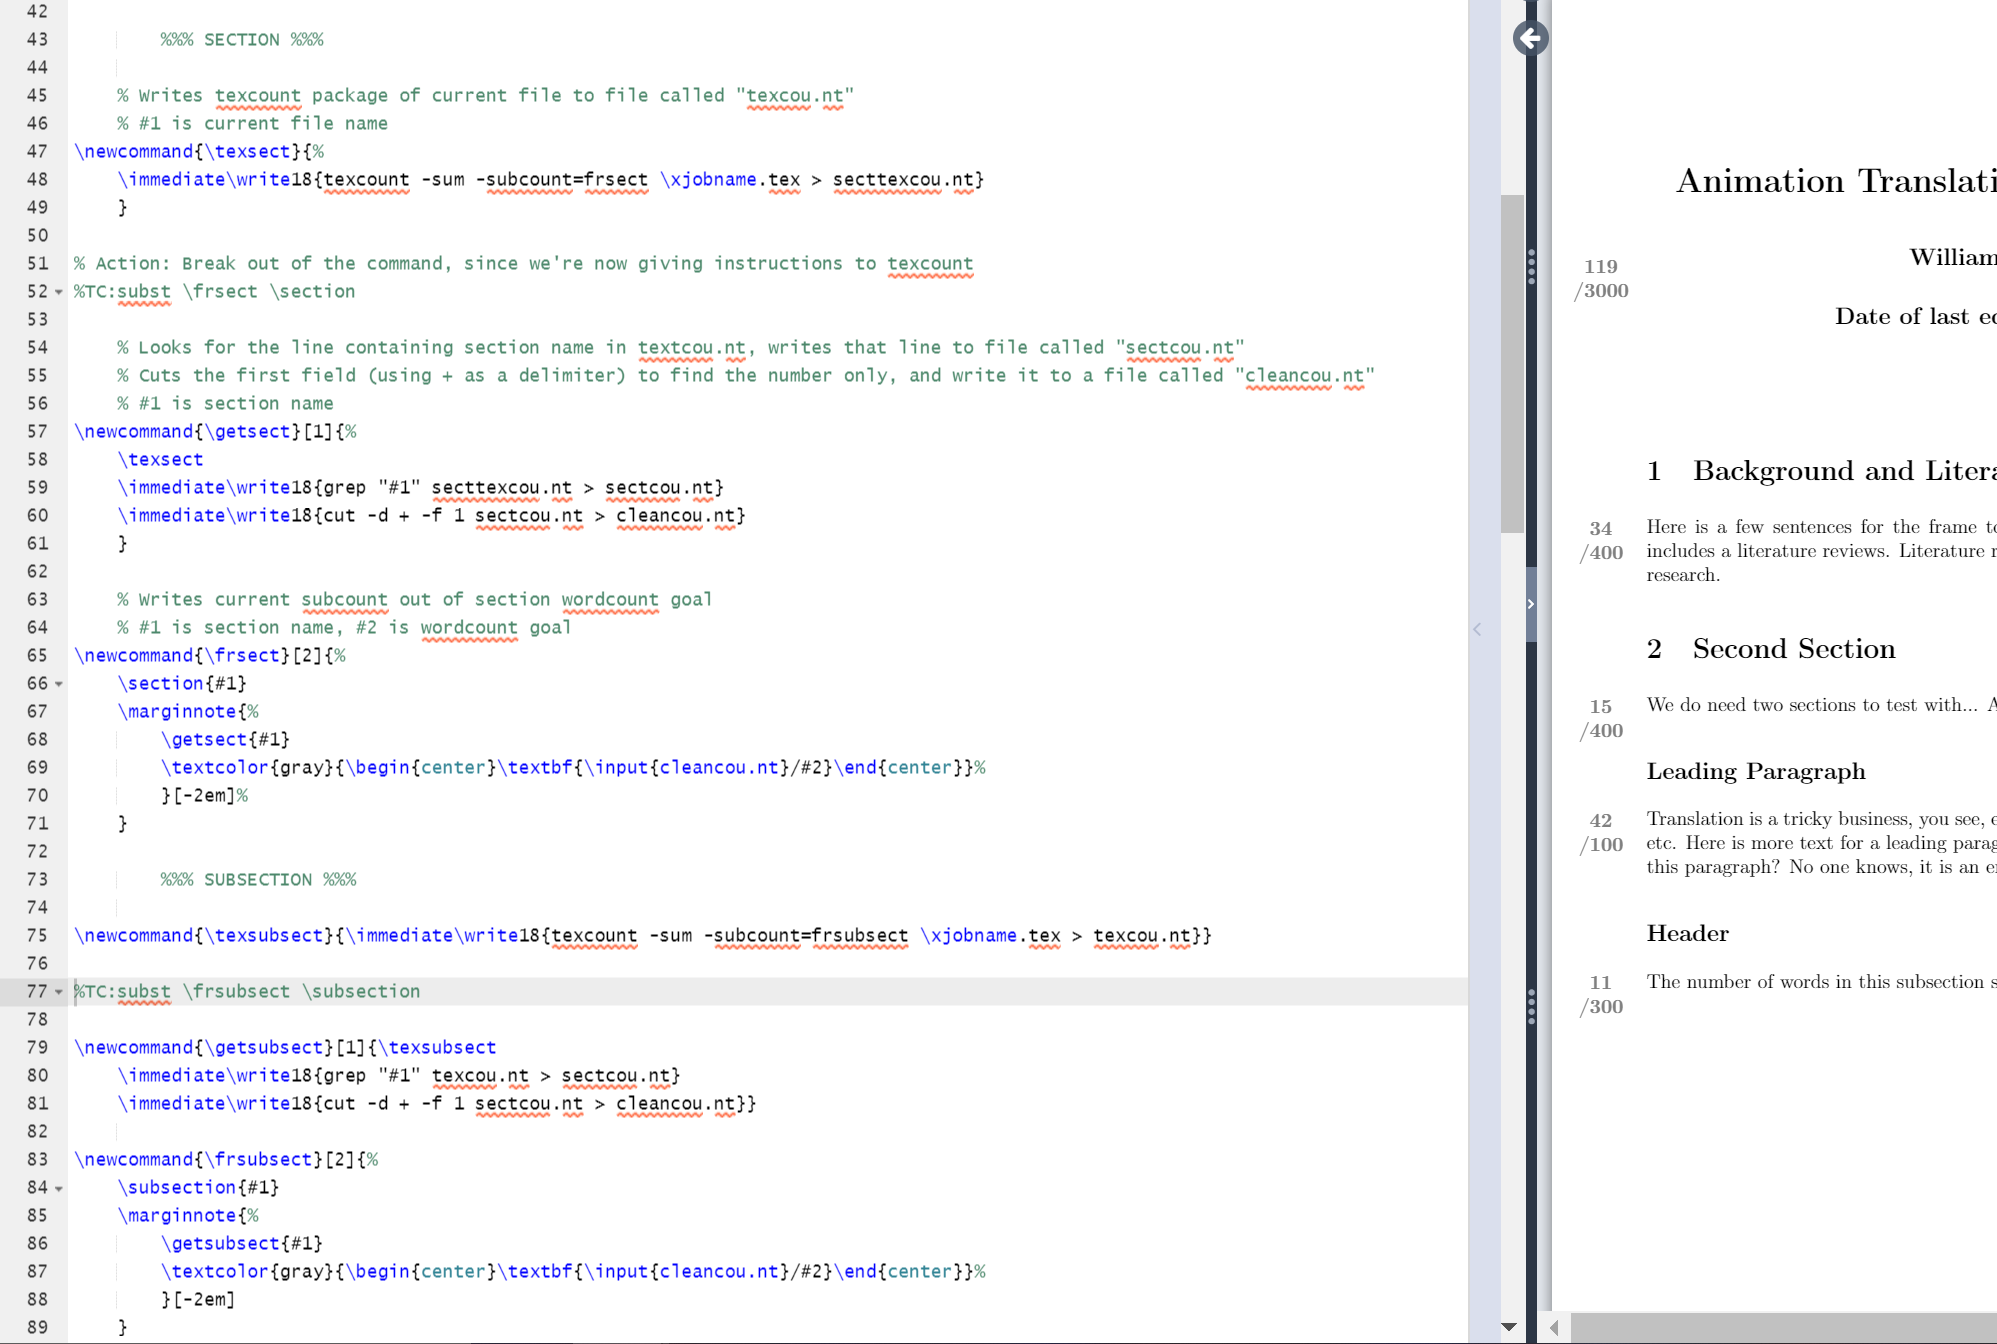
\includegraphics[width=\textwidth]{imgelaborationmargincount.PNG}

\newpage\underline{\textbf{\Large{Changing Frame Tests}}}

\section{\large Change colour of frame depending on frame contents}

\textbf{Intention:} Write conditionals for wordcount colouring using the \texttt{xcolor} package. At each recompile the wordcount should be blue within ten percent of the goal, orange within twenty percent of the goal, and red when over twenty percent. \href{https://en.wikibooks.org/wiki/TeX/ifnum}{This guide} to \texttt{ifnum} seems the easiest so far.

\textbf{Action:} \begin{verbatim}
     \marginnote{%
        \color{%
            \ifnum\input{cleancou.nt}>#2*1.3 Red%
            \else\ifnum(\input{cleancou.nt}-#2)/#2>0.1 BurntOrange%
            \else\ifnum\input{cleancou.nt}>#2*0.9 Blue%
            \else Gray%
            \fi\fi\fi}
            {\textbf{\input{cleancou.nt}\unskip/#2}}%
        }[-2em]%
\end{verbatim}

\textbf{Result:} Even with tinkering I seem to be a getting quite a few errors: 
\begin{enumerate}
    \item \texttt{$\backslash$input\{cleancou.nt\}} definitely isn't working within a macro. 
    \item \#2 also seems to be a problem, but \texttt{$\backslash$ifnum} is not accepting any attempts to put them in parentheses, brackets or braces.
    \item An error keeps appearing for \texttt{xcolor} that the colour ".3 Red" can't be found, and it's taking that decimal from a number I'm trying to use.
\end{enumerate}
Solutions:
\begin{enumerate}
    \item After reading a \href{https://tex.stackexchange.com/questions/204029/read-number-from-file}{tex.stackexchange of a similar problem}, I tried the same solution of opening and reading the file \texttt{cleancou.nt}, writing the number contained in the file to a defined as "\texttt{$\backslash$cnt}".
    \item Searched how to \href{https://tex.stackexchange.com/questions/67362/passing-argument-to-ifnum}{pass an argument to \texttt{ifnum}}, but the strategy employed does not seem to be working in this case at all. It's possibly due to then manipulating the number from the argument and working with that. I then looked up how to make calculations using arguments and found \href{https://tex.stackexchange.com/questions/453454/calculations-on-variables-using-latex}{this strategy} that uses the \texttt{xfp} package to create floating points. The example used \texttt{$\backslash$newcommand{$\backslash$areaHeatExchanger}{$\backslash$fpeval{$\backslash$lengthHeatExchanger * $\backslash$heightHeatExchanger}}} particularly seems to be analogous to what I need to do.
    \item Now that the previous issue is resolved, I can use these same floating points to keep manipulated numerals in braces, resolving the issue of decimal points accidentally being read as a colour. Unfortunately, because there is no manipulated number on the right side of the greater-than symbol, I'm still returning an error that the colour ".1 BurntOrange" is not a colour found in the \texttt{xcolor} package. Rather than bothering myself to create an argument or temporary file to get around that, I'll just change the maths to not require a decimal by multiplying both sides of the equation by 100.
\end{enumerate}

\textbf{Action:}
\begin{verbatim}
    \newread\tmp       
        \openin\tmp=cleancou.nt
        \read\tmp to \cnt
        \closein\tmp
    \marginnote{%
        \color{%
            \ifnum\cnt>\fpeval{#2*1.3} Red%
            \else\ifnum\fpeval{(\cnt-#2)/#2*100}>10 BurntOrange%
            \else\ifnum\cnt>\fpeval{#2*0.9} Blue%
            \else Gray%
            \fi\fi\fi}
            {\textbf{\input{cleancou.nt}\unskip/#2}}%
        }[-2em]%
\end{verbatim}

\textbf{Result:} Although this does actually compile, it brings up the same two error messages for nearly all instances where \texttt{$\backslash$frsect} is run: 
\begin{itemize}
    \item 
        \begin{verbatim}
        Missing = inserted for ifnum.
        <to be read again>
        l.143 ...ct{Background and Literature Review}{400}
        I was expecting to see `<', `=', or `>'. Didn't.
    \end{verbatim}
    \item 
    \begin{verbatim}
        Missing number, treated as zero.
        <to be read again>                           .
        l.143 ...ct{Background and Literature Review}{400}
        A number should have been here; I inserted `0'.
        (If you can't figure out why I needed to see a number,
        look up `weird error' in the index to The TeXbook.)
    \end{verbatim}
\end{itemize}

\textbf{Action:} Research is absolutely not helping. I've tried using \texttt{etoolbox}, removing one line of code at a time, changing what it should output, researching how to use \texttt{$\backslash$relax}, and the same two errors appear on all sections except the second one. Removing one line of code at a time revealed the problem is with the two \texttt{$\backslash$else$\backslash$ifnum} lines but I can find plenty of examples online of nesting \texttt{$\backslash$ifnum} without issue. The \textbf{action} here is just to keep "tinkering" until it works out.

\textbf{Result:} The issue turned out to be with \begin{verbatim}
    \else\ifnum\fpeval{(\cnt-#2)/#2*100}>10 BurntOrange%
\end{verbatim}
The problem was that some of the sections had more than one test being true/false this way. It was running them in order to compile, which is what I wanted, but it produced the errors.

I tinkered for five hours. 

\textbf{Action:} \begin{verbatim}
    \newcommand{\frsect}[2]{%
    \section{#1}
    \getsect{#1}
    \newread\tmp      
        \openin\tmp=cleancou.nt
        \read\tmp to \cnt
        \closein\tmp
    \marginnote{%
        \color{%
            \ifnum\cnt>\fpeval{#2*1.2} Red%
            \else\ifnum\cnt>\fpeval{#2*1.1} BurntOrange%
            \else\ifnum\cnt>\fpeval{#2*0.9} ForestGreen%
            \else Gray%
            \fi\fi\fi}
            {\doublebox{\large\textbf{\input{cleancou.nt}\unskip/#2}}}
        }[-2em]%
    }
\end{verbatim}

\textbf{Result:} 

\centering{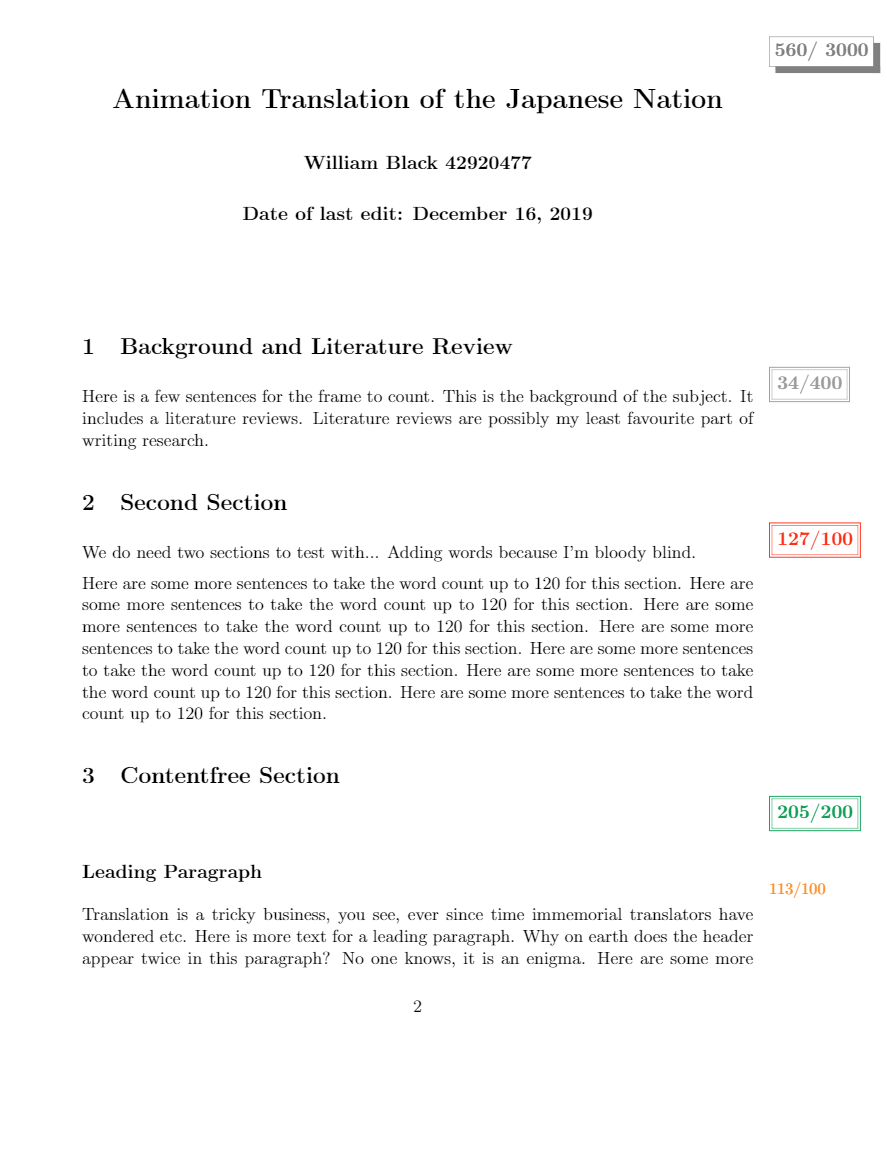
\includegraphics[scale=0.8]{imgelaborationcolourcount.PNG}}

\flushleft It completely and totally works. I'm not sure why I would have wanted it to be orange when \textit{approaching} the goal in the first place, but I'm happy to lose this feature. I could just add it in again for \texttt{>\{\#2*0.8\}} but I don't want it, the program is more useful without it. 


\section{\large Frames can be toggled on/off} 

\textbf{Intention:} Create a toggle for the macro. I've been looking up how to make an \href{https://www.overleaf.com/learn/latex/Writing_your_own_package#Preliminary_declarations}{option} for the macro to turn it off so I can see how the product will look when I remove the frame and export it as a .pdf. I found slightly more comprehensive instructions from someone looking to do something similar on a \href{https://tex.stackexchange.com/a/449385}{stackexchange board}. Having never heard of "booleans", I'm using a \href{https://tex.stackexchange.com/questions/101076/difference-between-newbool-and-newtoggle-from-etoolbox-package}{tangentially related stackexchange thread} to help guide me setting the boolean and using the option in the code.

\textbf{Action:}

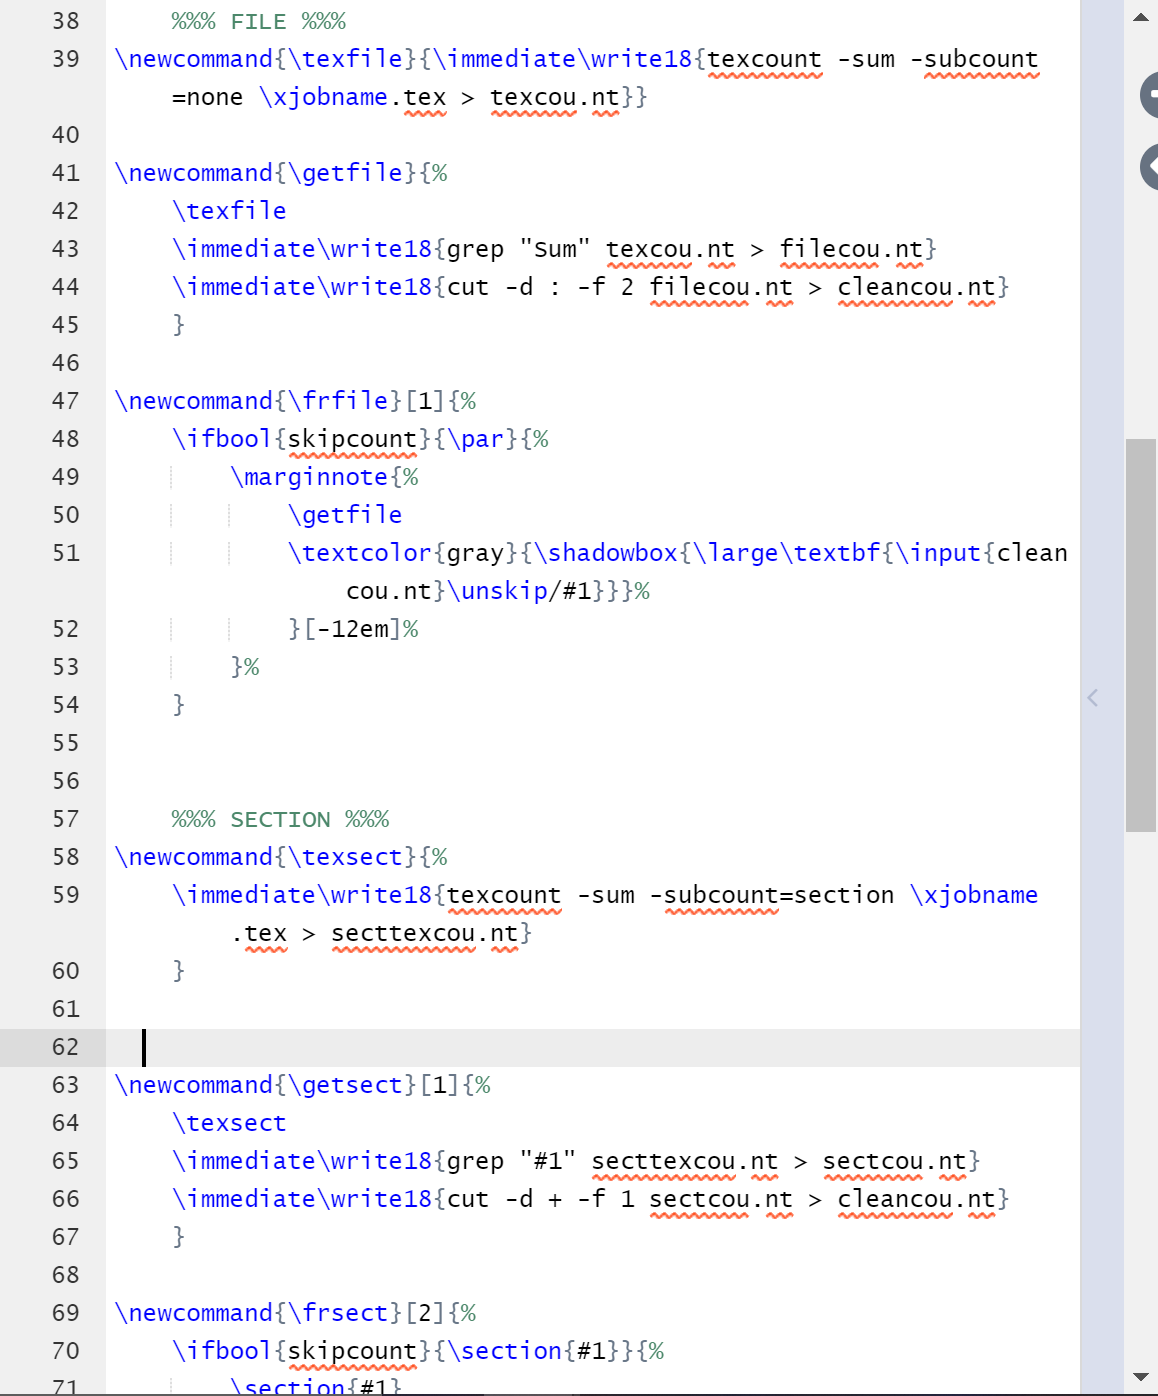
\includegraphics[scale=0.7]{imgelaborationbooleans.PNG}

\textbf{Results:} It didn't work until I moved the TexCount invocation back into the test document. That means that added to each preamble, the user will need to define \texttt{$\backslash$xjobname} and also write \texttt{\%TC:subst frsect section} and \texttt{\%TC:subst frsubsect subsection} in their own preamble. I will have to add that to the instructions.

\section*{\underline{Elaboration Results}}

The Proof of Concept has passed all necessary tests to prove it is feasible to build. In this instance, it was necessary to actually build the macro to test whether it would be feasible, and the finished product is currently functional as-is.

\end{document}
